\documentclass{article}


% if you need to pass options to natbib, use, e.g.:
    \PassOptionsToPackage{numbers, compress}{natbib}
% before loading neurips_2023


% ready for submission
% \usepackage{neurips_2023}


% to compile a preprint version, e.g., for submission to arXiv, add add the
% [preprint] option:
    \usepackage[preprint]{neurips_2023}


% to compile a camera-ready version, add the [final] option, e.g.:
    % \usepackage[final]{neurips_2023}


% to avoid loading the natbib package, add option nonatbib:
%    \usepackage[nonatbib]{neurips_2023}


\usepackage[utf8]{inputenc} % allow utf-8 input
\usepackage[T1]{fontenc}    % use 8-bit T1 fonts
\usepackage{hyperref}       % hyperlinks
\usepackage{url}            % simple URL typesetting
\usepackage{booktabs}       % professional-quality tables
\usepackage{amsfonts}       % blackboard math symbols
\usepackage{nicefrac}       % compact symbols for 1/2, etc.
\usepackage{microtype}      % microtypography
\usepackage{xcolor}         % colors
\usepackage{amsmath}
\usepackage{amssymb}
\usepackage{graphicx}

\usepackage{algorithm}
\usepackage{algorithmic}


\title{Meta-learning Implicit Neural Representation for Sparse Time Series Functional Data Analysis}


% The \author macro works with any number of authors. There are two commands
% used to separate the names and addresses of multiple authors: \And and \AND.
%
% Using \And between authors leaves it to LaTeX to determine where to break the
% lines. Using \AND forces a line break at that point. So, if LaTeX puts 3 of 4
% authors names on the first line, and the last on the second line, try using
% \AND instead of \And before the third author name.


% \author{%
%   David S.~Hippocampus\thanks{Use footnote for providing further information
%     about author (webpage, alternative address)---\emph{not} for acknowledging
%     funding agencies.} \\
%   Department of Computer Science\\
%   Cranberry-Lemon University\\
%   Pittsburgh, PA 15213 \\
%   \texttt{hippo@cs.cranberry-lemon.edu} \\
  % examples of more authors
  % \And
  % Coauthor \\
  % Affiliation \\
  % Address \\
  % \texttt{email} \\
  % \AND
  % Coauthor \\
  % Affiliation \\
  % Address \\
  % \texttt{email} \\
  % \And
  % Coauthor \\
  % Affiliation \\
  % Address \\
  % \texttt{email} \\
  % \And
  % Coauthor \\
  % Affiliation \\
  % Address \\
  % \texttt{email} \\
% }

\author{%
  Bofan Chen\\
  Department of Pure Mathematics and Mathematical Statistics\\
  University of Cambridge\\
  \texttt{cbfcbf.byron@gmail.com} \\}
\begin{document}


\maketitle

\begin{abstract}
  Sparse time series data are everywhere in our daily life. However it is hard to analyze them by traditional statistical methods. Here, we propose MetaINR, a method to learning the implicit neural representation (INR) given sparse obsevations of time series data.
  Based on this, estimations of mean function, covariance operator, and principal components can be implemented easily.
  The method introduce the meta-learning to the functional data analysis framework, which greatly outperforms the traditional baseline.
\end{abstract}

\section{Introduction}
Sparse time series data is prevalent in daily life, such as medical data measured at different times for patients or height data collected at various stages of adolescence. 
However, the sparsity and irregularity of such data make traditional statistical methods less suitable. 
Additionally, the consideration of continuity and differentiability properties in most time series data pose challenges for multivariable statistical analysis.

Recent research suggests that meta-learning exhibits great advantages in handling sparse data. 
It can learn commonalities among similar tasks, enabling few-shot learning or even one-shot learning on extremely sparse training sets. 
Besides, statistical analysis based on functional data has been hugely developed for dealing with continuous time series problems recently.

In this paper, we introduce a novel approach, metaINR, which combines meta-learning and functional data analysis to address the estimation challenges posed by sparse time series data. 
Through this method, we use meta-learning to realize the implicit neural representation (INR) to
reconstruct the time series function for each sample based on sparse time series observations.
Furthermore, we can estimate the mean, covariance, and principal components of the distribution of these samples.
Therefore, MetaINR method presents a fresh solution for addressing issues related to sparse time series data.

% Sparse time series data 在日常生活中非常常见,比如病人在不同时间测量的医疗数据、青少年在成长时不同阶段测量得到的身高数据等。这些数据的稀疏性和irregularity让传统的统计手段变得不太适用。同时,绝大多数时间序列数据所拥有的连续性,可微性等性质也给基于multivarible的统计学分析带来了困境
% 最近的研究表明,元学习在处理稀疏形数据中具有独特的优势。它可以从大量相似的任务中学习任务的共性,并对非常稀疏的训练集做到few-shot learning, 甚至 one-shot learning。同时,在处理连续的时间序列问题时,基于funcitonal data 的统计学也逐渐成熟。
% 在本文中,我们结合了meta-learning和functional data analysis的方法首次提出了metaINR,来解决对稀疏时间序列数据的估计问题。通过这个方法,我们可以基于多个样本的稀疏的时间序列观测较好地重构每个样本的时间序列函数,并且进一步地估算这些样本分布的均值、协方差和主成分。
% metaINR为处理稀疏时间序列问题给出了新的解决方案。
\section{Related works}

\subsection{Functional Data}

% Traditional multivariate statistics 把一个有限维空间中的向量作为研究对象,来分析它的统计性质,如均值向量、协方差矩阵等。在维度较小的时候,这并没有什么不妥。然而如果把分析对象所在空间的维度提高到无穷维,比如L2空间时,传统方法将会面临一些挑战。在函数空间,人们的关注点并不会局限于向量在某个维度上的取值,人们还会关注连续性、导数等更多性质。同时,随着空间增长到无穷维,原先多元统计中的很多指标也会丧失意义,如概率密度函数等。正是由于无穷维和有穷维空间的统计性质和人们关注点的不同,functional data analysis(FDA) 这个方向引起了研究者的广泛关注。
\textbf{Multivariate data versus functional data} 
Traditional multivariate statistics take finite-dimensional vectors as the objects of study to analyze their statistical properties, such as mean vectors and covariance matrices. 
This approach is appropriate and easy to compute when the dimension is relatively small. 
However, if the dimension of the space in which the objects are analyzed is increased to infinite, for example, in $L^2$ space, traditional methods face certain challenges. 
In such functional spaces, the focus is not only on the values of vectors in a particular dimension but also on properties such as continuity, smoothness and derivatives. 
At the same time, as the space grows to infinite dimensions, many useful tools in multivariate statistics, such as probability density functions, will lose their meaning. 
It is the differences in statistical properties and people's focus between infinite-dimensional and finite-dimensional spaces, that have led to widespread attention to functional data analysis (FDA) among researchers.

% Time series是一个很典型的需要在无穷维函数空间中处理的研究对象。这是因为现实中收集的时间序列数据往往具有连续性,同时,在某些情况下,人们会关注它的导数、时间对齐(registration)等话题。有很多之前的研究基于多元统计学对时间序列进行分析。比如···。从函数逼近的观点来看,这些基于多元统计的研究确实能够很好的反映一些时间序列的性质,但是这在很多情况下是比较难以推广的,比如本文中所研究的sparse time series data。
\textbf{Time series as a representative example of functional data}
Time series is a typical object that needs to be addressed in an infinite-dimensional function space. 
This is because time series data collected in reality often exhibit continuity, and, in certain situations, people may focus on topics such as derivatives and time alignment (registration).
Many previous studies have relied on multivariate statistics in the analysis of time series, such as \textcolor{red}{[mention some specific examples]...}
From the perspective of function approximation, these multivariate-statistics-based studies can indeed reflect certain properties of time series. 
However, in many cases, this approach is challenging to generalize, as is the case with sparse time series data studied in this paper.

% 当人们对time series的观测频率不高并且不规律的时候,就会形成sparse time series data。这种类型的数据在医学领域中尤其常见,因为人们只有在医院才会采集数据,而往往看病的次数是因人而异的,看病频率的也是不规律的。如果要用多元统计学分析这种类型的“杂乱”数据,人们往往会束手无策。在functional data analysis中,人们可以通过local polynomial regression的方法先估计出函数形数据的原始形式,然后在这个基础上估计均值,协方差算子等统计量(详见appendix)。local polynomial regression可以表示如下:
\textbf{Sparse times series data analysis}
When the observation frequency of time series is low and irregular, sparse time series data is formed. 
We can represent the sparse dataset of $n$ samples as 

where
$y_{ij}=x_i(t_{ij}) , i=1, \cdots, n, j=1, \cdots, J_i$ and $J_i$ is the total observations of the $i$-th sample.
This type of data is particularly common in the medical field, as the frequency of medical visits varies from person to person, with irregular patterns.
When it comes to analyzing such "messy" data using multivariate statistics, people often find themselves at a loss.
However, in functional data analysis, one can employ the method of local polynomial regression to estimate the mean function and covariance operator of functional data.
Specifically, given our sparse observations of dataset $D$,
we can define the loss function to estimate mean function $\mu(t)$
$$
L_t^\mu(\beta)=\sum_{i=1}^n\sum_{j=1}^{J_i}\left[y_{ij}-\sum_{r=0}^R \beta_r\left(t-t_{ij}\right)^r\right]^2 K\left(\frac{t-t_{ij}}{h}\right),
$$
where $K(\cdot)$ is the kernel function and $h$ is the bandwidth which shoud be carefully chosen based on data.
By minimizing this function, we can get
$\beta_t=(\beta_0(t), \cdots, \beta_R(t))=arg\,min L_t^\mu(\beta)$. The estimator of mean function cam be defined as $\hat{\mu}(t)=\beta_0(t)$.
Similarly, to estimate the covariance kernel $c(t,s)$, we define the loss function 
$$
L^c_{t,s}(\beta)=\sum_{i=1}^n \sum_{1\leq j, l, \leq J_i} K_{t,s}(\frac{t-t_{ij}}{h}, \frac{s-t_{il}}{h}) \left[ g(t_{ij},t_{il})-f\left(\beta,(t,s),(t_{ij},t_{il})\right) \right]^2
$$
where
$$
g(t_{ij},t_{il})=(y_{ij}-\hat{\mu}(t_{ij}))(y_{il}-\hat{\mu}(t_{il}))
$$
$$
f\left(\beta,(t,s),(t_{ij},t_{il})\right)=\beta_0 + \beta_{11}(t-t_{ij})+\beta_{12}(s-t_{il})
$$
By minimization of $L_{t,s}^c(\beta)$, we obtain $(\beta_0(t),\beta_{11}(t),\beta_{12}(t))=arg\,min L_{t,s}^c(\beta)$. Then the estimator of the covariance kernel is defined as $\hat{c}(t,s)=\beta_0(t)$.
Based on the estimation of mean and covariance,  we can use the method of Principal Analysis by Conditional Expectation (PACE) to reconstruct each sample and compute their scores \textcolor{red}{(see details in the appendix)[TODO]}.
Comparing to using local polynomial regression directly to reconstruct samples, It is noticeable that the reconstruction of the sample makes use of the total of information of all observations, but it hugely relies on the assumption that scores are normally distributed. 
\textcolor{red}{In the following text, I will compare the estimates obtained based on this method as the baseline with the meta-learning-based approach proposed in this paper.[TODO PACE baseline coding]} 
% 下文中我会将基于这种方法得到的估计值作为Baseline与本文提出的基于metalearning的方法相比较。

\subsection{Implicit Neural Representation}

% 传统上,函数形数据的表示会用标准的网格法,即给定有限个坐标和函数值的pairs(ti,yi)。这么做有一定的缺陷:原来在无穷维空间中的函数形数据被离散化到了有穷维空间,它不仅不利于求导等计算,而且会极大影响函数的在一个较小时间区间上的分辨率。随着深度学习的兴起,人们发现可以利用深度神经网络来表示函数。···
\textbf{Traditional grid-based representation versus implicit neural representation}
Traditionally, the representation of functional data $y(t)$ involves using a standard grid-based method, 
wherein a finite set of coordinates and corresponding function values are given as pairs $(t_i, y_i)$. 
However, this approach has certain drawbacks: the original functional data in an infinite-dimensional space is discretized into a finite-dimensional space. 
This not only hampers operations like differentiation but also significantly impacts the resolution of the function within a smaller time interval.
With the emergence of deep learning, it has been discovered that utilizing deep neural networks can be an effective way to represent functions implicitly.
Implicit neural representation (INR) parameterize the functional data by deep neural networks:
$$y(t)=F_\phi(t), $$
where $F_\phi(\cdot)$ is a deep neural network parameterized by $\phi$.
This type of continuous representation not only proves to be more memory-efficient but also enables higher resolution and the handling of more complex operations on functional data.

%【】提出了SIREN的函数结构,。
\textbf{SIREN architecture for time series}
% 很多之前的工作用Relu-based multilayer perceptrons(MLP) 来作为INR的神经网络架构,但是基于这种架构的INR往往缺乏表达信号中精细细节的能力,并且不能很好的表示目标信号的多阶导数。为了解决这个问题,【1】提出了SIREN的架构来替代传统的ReLU-MLPs。它使用sine函数来作为神经网络的激活函数,可以很好的刻画函数的细节。令人惊奇的是,当对用SIREN来表示函数求导后,它依然可以用SIREN来表示。虽然之前的研究大多利用SIREN来表示图像和视频,却很少用来表示时间序列。本文将SIREN用在时间序列的分析中,我们发现SIREN在表示时间序列上具有优越性。
Many prior works have utilized ReLU-based multilayer perceptrons (MLP) as the neural network architecture for Implicit Neural Representations (INR). 
However, ReLU-based INR often lack the ability to capture fine details in signal and struggle to effectively express higher-order derivatives.
In addressing this limitation, \cite{sitzmann2020implicit} introduced the SIREN architecture as an alternative to traditional ReLU-MLPs:
$$
\Phi(\mathbf{x})=\mathbf{W}_n\left(\phi_{n-1} \circ \phi_{n-2} \circ \ldots \circ \phi_0\right)(\mathbf{x})+\mathbf{b}_n, \quad \mathbf{x}_i \mapsto \phi_i\left(\mathbf{x}_i\right)=\sin \left(\mathbf{W}_i \mathbf{x}_i+\mathbf{b}_i\right)
$$
SIREN employs the sine function as the activation function, effectively capturing intricate details in functions.
A remarkable observation is that even after taking derivatives of a function represented using SIREN, 
it can still be expressed using the SIREN architecture. 
While previous research predominantly applied SIREN to represent images and videos, its application in time series representation has been limited. 
This paper explores the utilization of SIREN in the analysis of time series and demonstates its superiority in time series INR.

\subsection{Meta-learning}

\textbf{Meta-learning framework}
Meta-learning was initially introduced to enhance the efficiency of machine learning, often referred to as ``learning to learn''.
By employing the deep learning model $F_\phi(\cdot)$ to address similar tasks, the ``shared characteristics'' among these tasks can be leveraged to expedite the machine learning process. 
% Meta-learning 一开始被提出是为了提高机器的学习效率,即learning to learn。 使用同一个模型来解决一系列相似的task,往往可以利用这些相似任务的”共性“来帮助机器更快地完成训练。
To fomulate, given the observation dataset $D^*$ of the target task and the observation dataset $D=\bigcup_{i=1}^n D_i$ of $n$ similar tasks, we need to find a meta-function to effectively learn the parameters of the given task, namely $\phi^*=f_\theta(D,D^*)$,
where $\theta$ is the meta-parameter of the meta-function $f_\theta(\cdot)$. Accordingly, the original target task can be solved as $F_{\phi^*}(\cdot)$.
In fact, the representation of meta-function $f_\theta(\cdot)$ can be diverse. There are two main classs of methods:  Parameterized Policy Gradient Methods (PPG) and Black Box Methods.

\textbf{Parameterized Policy Gradient Methods and MAML}
The PPG method use an iterative algorithm to represent $f_\theta$, which has an innerloop of the form:
$$
\phi^*_{j+1}=\phi_j^*-\alpha_\theta \nabla_{\phi_j^*} \hat{L}_\theta\left(D^*, F_{\phi_j^*}\right),
$$
with the initial value $\phi_0^*=\phi_0^*(\theta)$.
This is very intuitive because it is similar to the traditional gradient decent method to optimize. 
The only difference is that $\theta$ should be carefully determined by the observations of other tasks $D$ in this scenario.
One important example of PPG method is MAML, where $\phi_0^*(\theta)=\theta$ and $\hat{L}_\theta$ can be any loss function independent of $\theta$.
MAML can be regard as learning an initial value for a task distribution, which retains the gradient decent framework of traditional optimization algorithms.


\textbf{Black Box Methods}
Since we only care about the target function $F_\phi(\cdot)$ rather than the value of parameters $\phi$, an alternative way to treat $f_\theta(\cdot)$ is to see it as a black box. Based on this idea, we can rewrite the target function:
$$
F_\phi(t)=F_{f_\theta(D,D^*)}(t)=g_\theta(t,D,D^*)
$$
Here we do not need to explicitly specify the value of $\phi$, and treat the meta-learning task as another ``big'' task, which adds all the training materials into input.
Because of the sequential properties of the datasets, sequential model architectures such as RNN are used in $g_\theta$, which unavoidably change the initial architecture $F_\phi$.
In contrast, PPG methods use the meta-parameters $\theta$ to find the task parameters $\phi$ explicitly, which maintain the initial network architecture.
Therefore, black box methods have inductive bias from data while PPG methods have inductive bias in network structure.

In the context of time series Implicit Neural Representation (INR), selecting an appropriate network structure is crucial, as it directly influences properties such as continuity and differentiability.
Hence, in this paper, we opt for MAML as our meta-learning method for the INR task.

\section{Method}

\textbf{Overview of MetaINR}
% 给定sparse observations of n similar time series, 我们的目标是尽可能的还原每一个sample并找到描述这一系列时间序列的主成分PC。
Given sparse observations of $n$ similar time series, the goal of MetaINR is to reconstruct each sample as accurately as possible and identify the principal components (PC) of these time series.
% As discussed in the previous section,在传统的方法中,我们首先利用local polinomial regression 估计这些时间序列的均值和方差,在scores服从正态分布的条件下,就可以利用PACE的方法估计出每个主成分并reconstruct each sample.
As discussed in the previous section, in traditional approaches, we first use local polynomial regression to estimate the mean and covariance of these time series. 
Under the assumption that scores follow a normal distribution, the PACE method can then be employed to estimate each principal component and reconstruct each sample.
% 这种两步估计的方法固然优于直接利用local polynomial 重构sample, 因为它利用了所有样本的信息。但是它依然存在两大明显的缺点:1. scores 服从正态分布的假设太强;2. 均值和协方差的估计不一定准确。
While this two-step estimation method is indeed superior to directly reconstructing samples using local polynomials as it leverages information from all samples, it still has the notable drawback that 
the assumption that scores follow a normal distribution is too restrictive.
% 在我们的方法中,我们不把meta-learning看成是一种高效学习的方法,而把他当作一种学习大量任务中共性的手段。 利用这个性质,我们先通过meta learning来学习出给定的多个timeseries的共性,然后基于共性还原每个sample的INR。再根据每个sample的INR得到均值和方差的估计值。最后利用方差核来估计主成分。
Here, we choose an alternative way by using the method of meta-learning, which involves three main steps:
\begin{itemize}
  \item Learning the meta-model: use SIREN architecture and MAML algorithm to learn the meta-model for the INR of given time series.
  \item Recovery of samples: calculate the SIREN-based INR efficiently for each time series sample based on the mata-model.
  \item Functional data estimation: use INR of each sample to estimate the mean function, covariance kernel and principal components.
\end{itemize}
We now discuss each step.

\textbf{Learning the meta-model}
The tasks here are realizing the implicit neural representation of samples by the SIREN architecture $F_\phi(t)$.
Given the sparse observations of $n$ similiar time series $D=\{(t_{ij},y_{ij})_{j=1}^{J_i}\}_{i=1}^n$,
we use MAML algorithm \ref{MAML} to learning the meta-model of these tasks, 
whose initial value of parameters are denoted by $\phi_0$. 
The MAML optimization process to find $\phi_0$ can be expressed as follows:
\begin{algorithm}
	\renewcommand{\algorithmicrequire}{\textbf{Input:}}
	\renewcommand{\algorithmicensure}{\textbf{Output:}}
	\caption{Model-Agnostic Meta-Learning for Time Series Implicit Neural Representation}
	\label{MAML}
	\begin{algorithmic}
    \REQUIRE $D=\{(t_{ij},y_{ij})_{j=1}^{J_i}\}_{i=1}^n$: the sparse observations for tasks
    \REQUIRE $\alpha, \beta: \text { step size hyperparameters }$
		\STATE randomly initialize $\theta$
    \WHILE {not done} 
      \FOR{all $i$}
        \STATE $\theta^0 \gets \theta$
        \FOR{$q = 0$ to $Q-1$  }
          \STATE Evaluate $\nabla_{\theta^q} \mathcal{L}_{i}\left(F_{\theta^q}\right)$ using support set $D_i^{\text{support}}=(t_{ij},y_{ij})_{j=1}^{\lfloor 0.5*J_i\rfloor }$
          \STATE Compute adapted parameters with gradient descent:
          $\theta_i^{q+1}=\theta_i^q-\alpha \nabla_{\theta_i^q} \mathcal{L}_{i}\left(F_{\theta_i^q}\right)$
        \ENDFOR
        \STATE Compute the loss $\mathcal{L}_{i}\left(F_{\theta_i^Q}\right)$ in sample $i$ using query set $D_i^{\text{query}}=(t_{ij},y_{ij})_{j=\lfloor 0.5*J_i\rfloor }^{J_i}$
      \ENDFOR
      \STATE Compute the total loss $\mathcal{L} = \sum_{i=1}^n \mathcal{L}_{i}\left(F_{\theta_i^Q}\right)$
      \STATE Update meta-parameters $\theta \leftarrow \theta-\beta \nabla_\theta \mathcal{L} $
    \ENDWHILE 
    \STATE $\phi_0 \gets \theta$
		\ENSURE the meta-parameters $\phi_0$
  \end{algorithmic}  
\end{algorithm}

\textbf{Recovery of samples}
Based on this meta-model, we can use gradient decent algorithm\ref{INR-learning} to calculate the optimal parameters $\phi^*_i$ for the sample $i$ and hence obtain the INR $F_{\phi^*_i}(t)$. 
\begin{algorithm}
	\renewcommand{\algorithmicrequire}{\textbf{Input:}}
	\renewcommand{\algorithmicensure}{\textbf{Output:}}
	\caption{Implicit Neural Representation Learning for Target Sample}
	\label{INR-learning}
	\begin{algorithmic}
    \REQUIRE $D^*=(t_{ij},y_{ij})_{j=1}^{J^*}$: the sparse observations for the target task
    \REQUIRE $\alpha: \text { step size hyperparameters }$
		\STATE initialize $\phi \gets \phi_0$
    \WHILE {not done} 
      \STATE Evaluate $\nabla_{\phi} \mathcal{L}\left(F_{\phi}\right)$ using support set $D^*=(t_{j}^*,y_{j}^*)_{j=1}^{J^*}$
      \STATE Update parameters with gradient descent:
      $\phi=\phi-\alpha \nabla_{\phi} \mathcal{L}\left(F_{\phi}\right)$
    \ENDWHILE 
    \STATE $\phi^* \gets \phi$
		\ENSURE $\phi^*$: the parameters of INR for the target model 
  \end{algorithmic}  
\end{algorithm}

\textbf{Functional data estimation}
Based on the estimated INR $\hat{y}_i(t)=F_{\phi^*_i}(t)$, we subsequently estimate the mean function $\hat{\mu}(t)$ and covariance kernel $\hat{c}(t,s)$ as follows:
$$
\hat{\mu}(t)= \frac{1}{n} \sum_{i=1}^n \hat{y}_i(t)
$$
$$
\hat{c}(t,s)= \frac{1}{n} \sum_{i=1}^n  [\hat{y}_i(t))-\hat{\mu}(t)] [\hat{y}_i(s)-\hat{\mu}(s) ]
$$
According to the covariance operator, we can further estimate its principal components $\hat{\phi}_k$ by calculate the eigenfunctions of $\hat{c}(t,s)$.

In our approach, we view meta-learning not merely as an efficient learning method but as a means to learn commonalities among a large number of tasks.
Leveraging this property, the metaINR $\hat{y}_i(t)=F_{\phi^*_i}(t)$ implicitly contain the information of the whole datasets.
Consequently, it provides a robust estimation for sparse time series data.
\begin{figure}
  \centering
  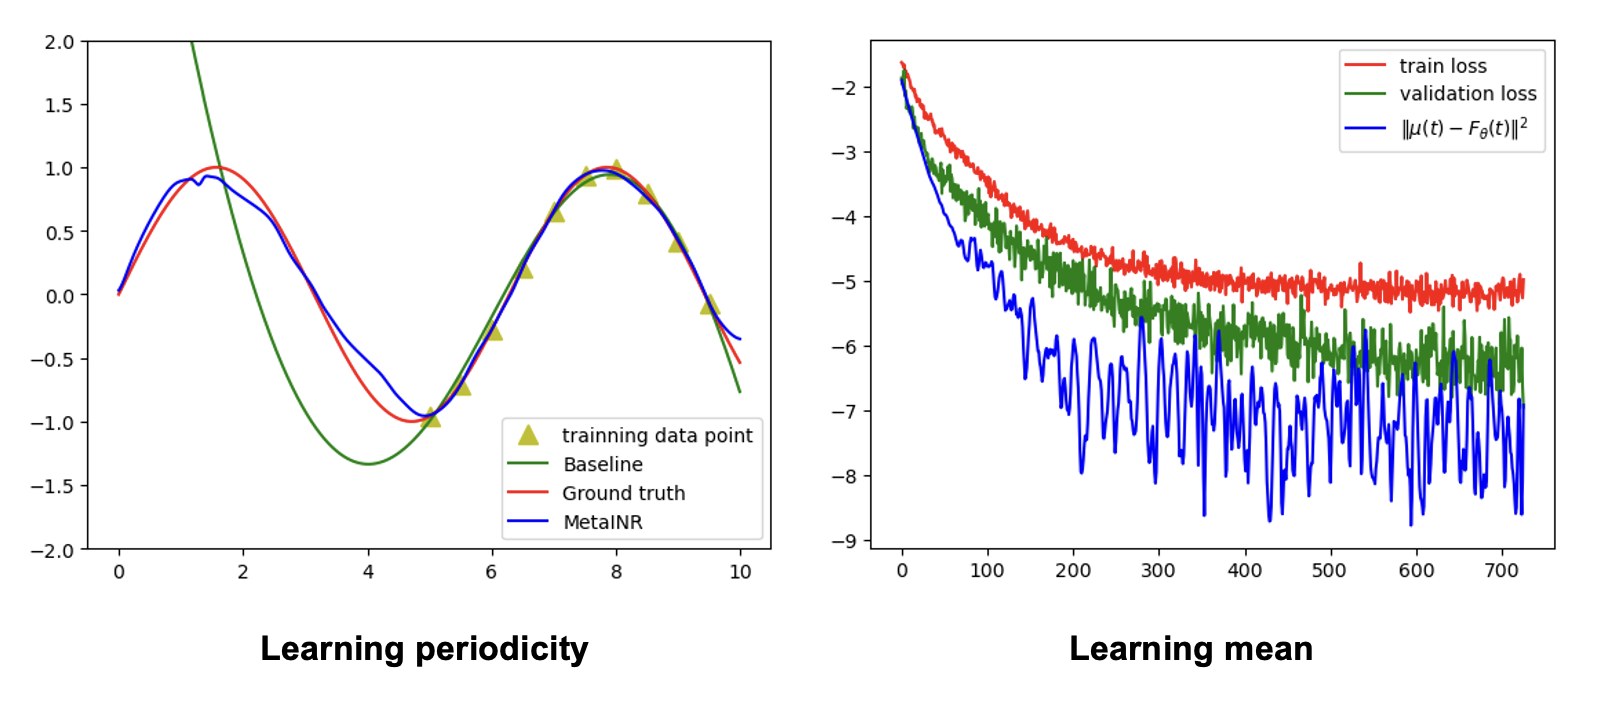
\includegraphics[width=\textwidth]{learning_commonalities.png}
  \caption{Learning commonalities}
  \label{Learning commonalities}
\end{figure}

\section{Experiments}
We evaluate our method on the synthetic data, with benchmark estimations provided by local polynomial regression \textcolor{red}{and the traditional PACE method [TODO]}.
Our results clearly demonstrate that MetaINR significantly outperforms the conventional baseline. 
Moreover, we extended our analysis to a real-world medical dataset to validate the robustness and applicability of our approach in practical scenarios.
% define evaluation method , measures? not only pictures
\subsection{Synthetic data}

\textbf{Data generating process}
Our ground truth of our synthetic data distribution is given by:
$$
y(t)=A sin(t)+ B sin(2t), \quad t \in [0,10],
$$
where $A$ and $B$ are independent and follows the uniform distribution
$$
A \thicksim Uniform[0,1], \quad B \thicksim Uniform[0,0.5].
$$
We randomly draw $n=100$ sample tasks $\{y_i(t)\}_{i=1}^n$ from this distribution.
For each sample task, $J=20$ observations randomly chosen in irregular time points.
The overall dataset employed for meta-learning comprises these observations.
$$
D=\{(t_{ij},y_{ij})_{j=1}^{J}\}_{i=1}^n
$$
% For training purposes, we further randomly divide overall dataset into training dataset and validation dataset, and for each sample task we randomly divide their observations into support and query sets. 
% $$
% D=\{(t_{ij},y_{ij})_{j=1}^{J}\}_{i=1}^n
% $$
\textbf{Meta-learning the commonalities of time series}
% 当我们对这个人造数据集进行元学习时,确实发现了元学习能够学习到一系列相似时间序列数据的共性。如图一所示,我们发现,当仅仅给出某一个样本后半段【5,10】这段区间的观测时,元学习能够从其他样本的数据中获得信息,学习到这个分布所包含的周期性。而local polynomial regression则仅仅基于单个样本的数据进行估计,这对于时间序列前半段的估计是不准确的。
When conducting meta-learning on this synthetic dataset, we indeed observed the capability of meta-learning to capture commonalities among a series of similar time-series data.
As shown in Figure \ref{Learning commonalities}a, we found that when providing observations solely for the latter segment ($t \in [5, 10]$) of a particular sample, 
meta-learning could extract information from data of other samples, learning the periodicity inherent in this distribution. 
In contrast, local polynomial regression relies solely on the data of an individual sample for estimation, 
resulting in less accurate predictions for the first half ($t \in [0, 5]$) of the time series.
% 除此之外,我们还发现metamodel中蕴含着均值的信息。当我们把MAML学习到的初始值直接带入SIREN模型形成我们的进一步学习的meta-model,我们发现meta-model与这些sample的均值及其接近。从图2中可以看到,元学习的过程同时伴随着元模型向均值逼近。
In addition, we discovered that the meta-model inherently contains information about the mean. 
By directly plugging the initial values learned by MAML into the SIREN model to construct our meta-model for further learning,
we observed a notable proximity between the meta-model and the means of these samples. 
As demonstrated in Figure \ref{Learning commonalities}b, the meta-learning process is accompanied by the meta-model gradually converging towards the mean.
% 除了这两个例子之外,【2】向我们展示了MAML能够加速学习的原因是feature reuse,这也解释了为什么元模型会包含数据集的多种特征。因此通过MetaINR进行基于稀疏观测的重建会比local polynomial regression 更加可靠。
Aside from these two examples, \cite{raghu2019rapid}  illustrates that MAML accelerates learning through feature reuse.
This also clarifies why the meta-model encompasses various features of the dataset. 
Consequently, employing MetaINR for time series reconstruction based on sparse observations proves to be more reliable than local polynomial regression.


% \begin{figure}
%   \centering
%   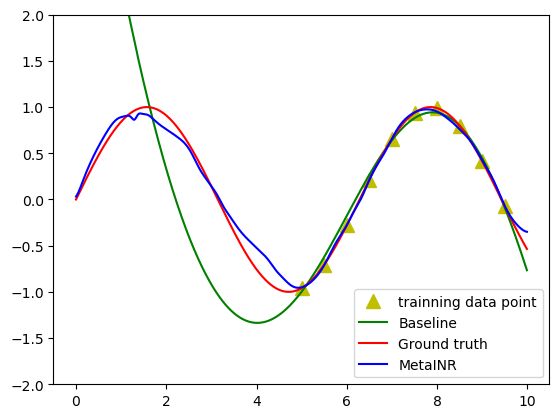
\includegraphics[width=0.5\textwidth]{learning_periodicity.png}
%   \caption{Learning periodicity}
% \end{figure}

% \begin{figure}
%   \centering
%   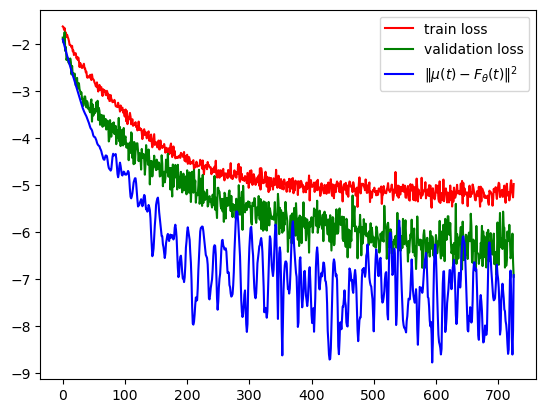
\includegraphics[width=0.5\textwidth]{learning_mean_loss.png}
%   \caption{Learning mean}
% \end{figure}

\textbf{Estimation of mean, covariance and principal components}
% 基于每个样本的MetaINR, 我们对这个人造数据集的均值函数,方差核和主成分进行了估计,结果如图3,4,5所示。
% 我们发现,以MetaINR为基础对三者的估计都远好于benchmark。特别是在数据的边界处,即t接近0或10的位置,baseline的估计往往与真实值相差甚远,而基于MetaINR的估计却相对可靠。
Based on MetaINR for each sample, we estimated the mean function, covariance kernel, and principal components of this synthetic dataset. 
The results are demonstrated in Figure \ref{Estimation for synthetic data}.
We observed that the estimators based on MetaINR for all three metrics significantly outperformed the benchmark. 
Particularly at the boundaries of the data, where $t$ approaches $0$ or $10$, 
the baseline estimators often deviated substantially from the true values,
while the estimateors based on MetaINR remained relatively reliable.

\begin{figure}
  \centering
  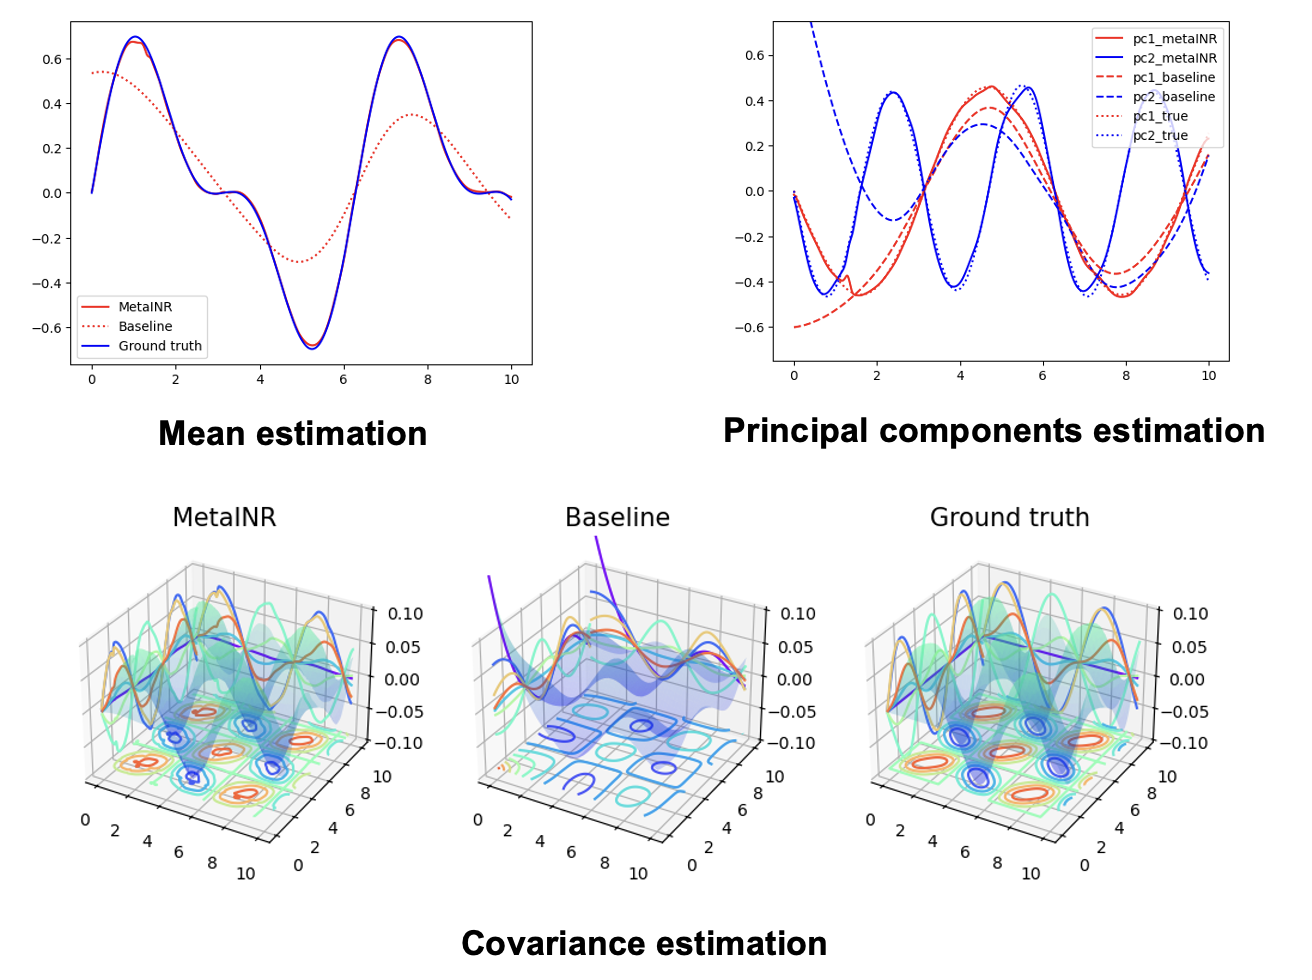
\includegraphics[width=\textwidth]{estimation.png}
  \caption{Estimation for synthetic data}
  \label{Estimation for synthetic data}
\end{figure}

% \begin{figure}
%   \centering
%   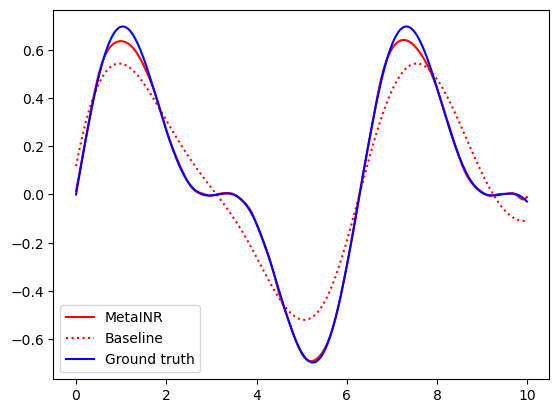
\includegraphics[width=0.5\textwidth]{mean.png}
%   \caption{Mean estimation}
% \end{figure}

% \begin{figure}
%   \centering
%   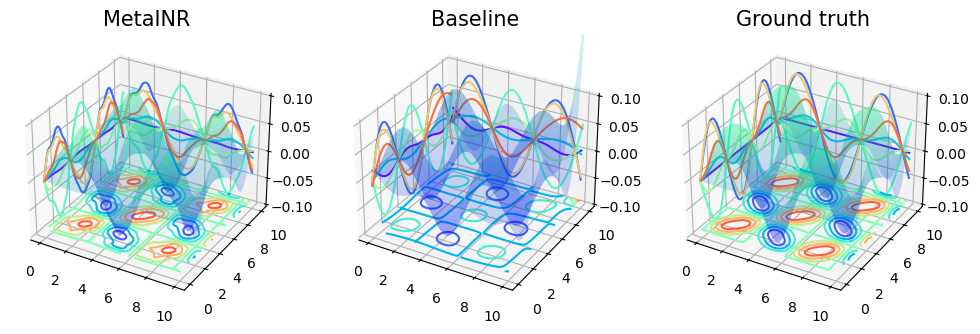
\includegraphics[width=\textwidth]{covariance.png}
%   \caption{Covariance estimation}
% \end{figure}

% \begin{figure}
%   \centering
%   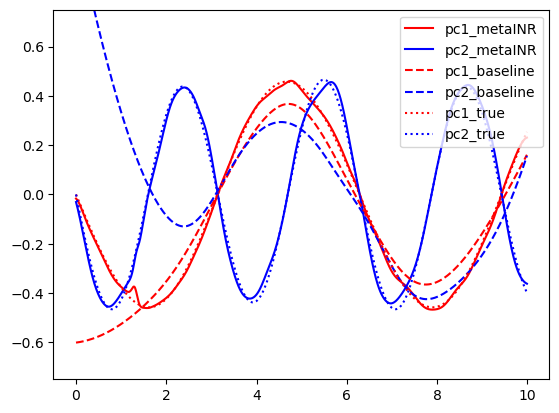
\includegraphics[width=0.5\textwidth]{fPCA.png}
%   \caption{FPCA}
% \end{figure}

%有待考虑
% \subsubsection{Metalearning+PACE Representation(dimensional reduction)}
% \subsubsection{Registration}

\subsection{Real-world data}
%CD4 count 的数据最好用
\textbf{Data description} 
We apply MetaINR to the longitudinal data on primary biliary cirrhosis (PBC).

\textcolor{red}{The data resulted from a Mayo Clinic trial that was conducted in 1974 to 1984. 
They are available at http://lib.stat.cmu.edu/datasets/pbc and have been described in Fleming \& Harrington (1991) and Murtaugh et al. (1994).
The data contain various sparsely and irregularly sampled covariates, 
as well as the survival or censoring time for each of 312 patients. 
Among these medical measurements ,
serum bilirubin concentration is known to be elevated in the presence of chronic liver cirrhosis, such as PBC.
}
We extracted data from the dataset for the initial 910 days, 
analyzing bilirubin measurements (in mg/dl) for different patients 
during the pre-onset phase. 
The goal was to characterize the pattern of this measurement over time through estimates of mean function, covariance kernel and principal components.
In the practice, we applied a logarithmic transformation to the bilirubin measurements and removed data for patients with a survival time less than 910 days.
% 因此,我们从数据集中截取了前910天的数据,对这发病前期不同病人的bilirubin measurements (in mg/dl)进行分析,期望通过主成分和均值的估计来刻画这个指标随时间变化的规律。
% 在实际操作中我们对bilirubin measurements取了对数变换,并且删除了存活时间小于910天的病人的数据。
A total of 260 patients in the study satisfied these criteria and only 2.9 observations per sample on average. 

\textbf{Estimation of mean, covariance and principal components}
% 如图3展示了MetaINR在实际sparse functional dataset中的估计结果。我们发现虽然每个样本只有极少数的观测点,但是MetaINR却能较好地恢复样本。在统计量的估计方面,在这个特定的实际数据集中,metaINR有着与Baseline类似的估计效果。我们可以通过估计结果得到如下结论:在前910天的观测中,病人的serum bilirubin concentration先小幅下降,在400天左右,它又急剧上升(mean function)。不同病人之间serum bilirubin concentration除了在基础值上有差异外(pc1),从400天左右, 病人的serum bilirubin concentration之间出现较大的分化差异(pc2)。
Figure \ref{Estimation for real-world data} illustrates the estimation results of MetaINR on the real-world medical sparse functional dataset mentioned above. 
We observe that despite the minimal number of observations per sample, 
MetaINR can effectively recover the sample function. 
Regarding the estimation of statistical quantities, 
MetaINR demonstrates similar performance to the baseline in this specific real dataset.
From the estimation results, we draw the following conclusions: 
Over the initial 910 days of observation, patients' serum bilirubin concentration initially experiences a slight decrease, 
followed by a sharp increase around 400 days (mean function). 
Apart from differences in ``baseline values'' which remain invariant with time (PC1), 
significant divergence in serum bilirubin concentration among patients emerges around 400 days (PC2).

\begin{figure}
  \centering
  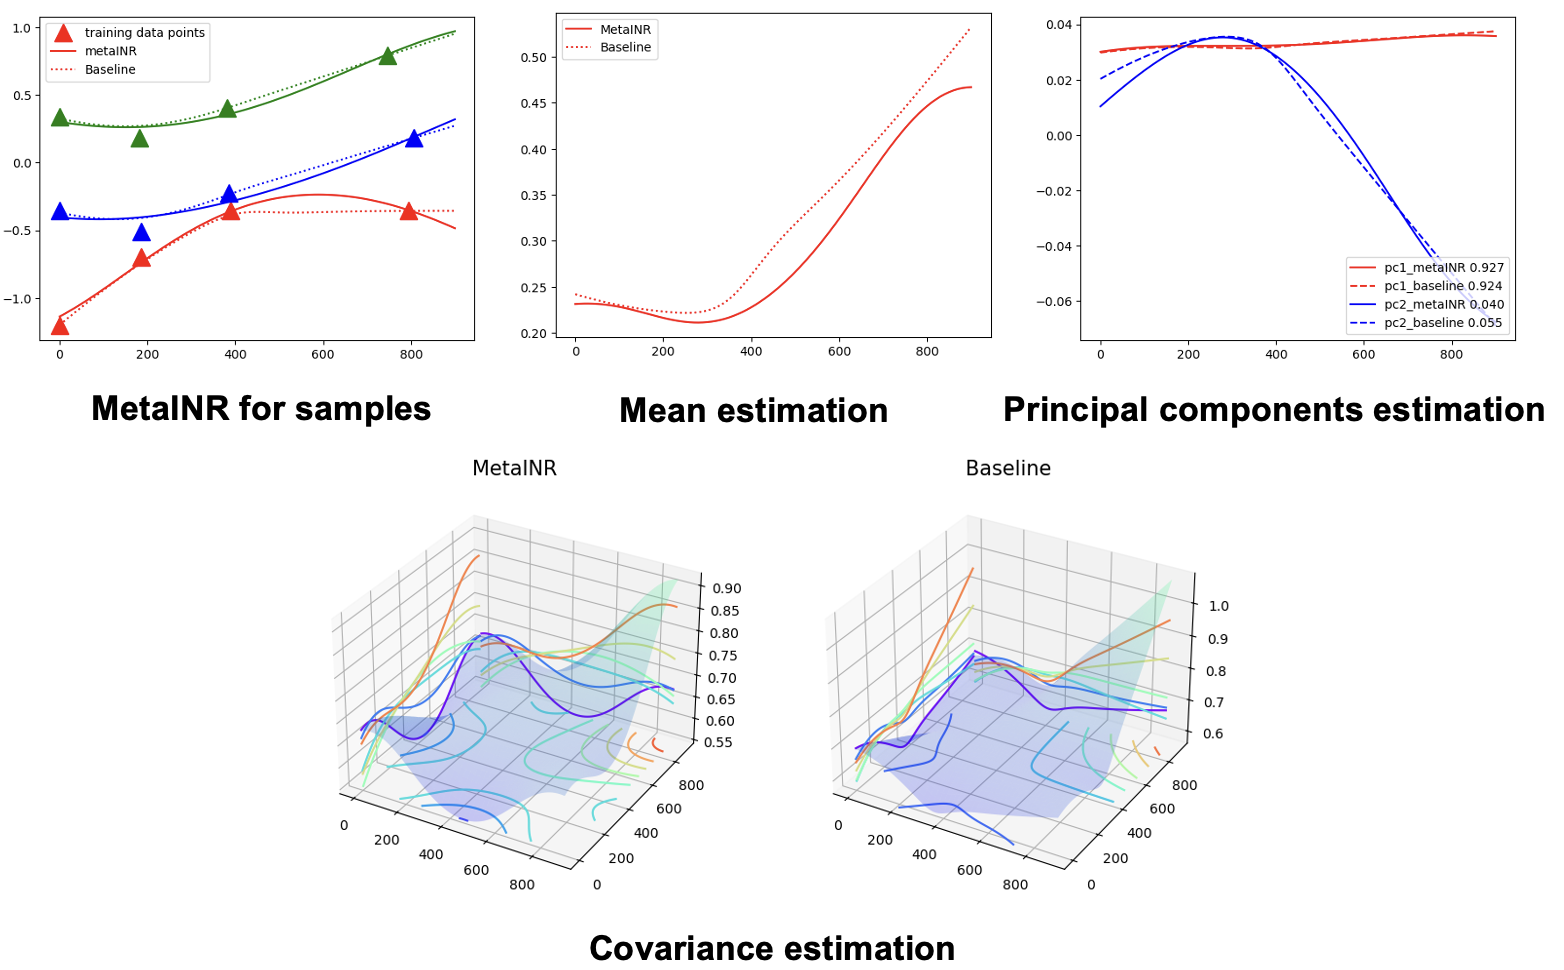
\includegraphics[width=\textwidth]{estimation_realData.png}
  \caption{Estimation for real-world data}
  \label{Estimation for real-world data}
\end{figure}

\section{Conclusion and future work}
% 我们展示了一个利用meta-learning的技术来处理sparse time series data的一个方法。通过meta-learning利用整个数据集的信息可以对只存在极少数观测点的样本进行MetaINR。基于MetaINR让一些原本只在稠密数据集中使用的functional data analysis的方法在sparse 数据集中变得可行。基于MetaINR的估计也为我们进一步分析sparse time series data提供了强大的工具。
We have shown a method named MetaINR utilizing meta-learning techniques to analyze sparse time series data. 
Through meta-learning, the MetaINR approach enables the estimation of functional form samples with very few observation points by leveraging information from the entire dataset. 
The application of MetaINR makes functional data analysis (FDA) methods, which are typically used in dense datasets, feasible for sparse datasets. 
Therefore, MetaINR provides a novel tool for further analyzing sparse time series data.
% 在未来的研究中,我们希望可以利用MetaINR对其他原本只适用于稠密数据集的funcational data analysis的方法进行拓展,如FPLS,functional regression等。从而结合MetaINR和FDA的方法来建立针对sparse data的分析工具库。

In future research, we aim to extend the application of MetaINR to other functional data analysis methods that were initially designed for dense datasets, such as Functional Partial Least Squares Regression (FPLS), functional regression, registration and more.
This approach aims to build an analytical toolkit for sparse data by combining MetaINR with various functional data analysis methods.
\section{Appendix}

\subsection{Traditional FDA method for sparse functional data: PACE}

\subsection{Brief introduciton to SIREN}

\subsection{Experiments on other synthetic data}


\bibliographystyle{IEEEtran}      %IEEEtran为给定模板格式定义文件名
\bibliography{ref}



% \section{Submission of papers to NeurIPS 2023}

% \begin{tabular}{c|ccc|ccc|ccc}
%   \toprule
%   & \multicolumn{3}{c}{Action Delay~$\tau=\bar{\Delta}$ s}      & \multicolumn{3}{c}{Action Delay~$\tau=2\bar{\Delta}$ s}      &  \multicolumn{3}{c}{Action Delay~$\tau=3\bar{\Delta}$ s}               \\
%           Dynamics Model                  & Cartpole & Pendulum & Acrobot                   & Cartpole & Pendulum & Acrobot                     & Cartpole & Pendulum & Acrobot \\        
%   \midrule
%   Random & 0.0$\pm$0.0 & 0.0$\pm$8.39 & 0.0$\pm$9.06 & 0.0$\pm$0.0 & 0.0$\pm$0.0 & 0.0$\pm$8.11 & 0.0$\pm$0.0 & 0.0$\pm$8.91 & 0.0$\pm$0.0 \\
%   \midrule
%   Oracle & 100.0$\pm$0.03 & 100.0$\pm$2.94 & 100.0$\pm$1.8 & 100.0$\pm$0.04 & 100.0$\pm$2.6 & 100.0$\pm$2.19 & 100.0$\pm$0.11 & 100.0$\pm$1.52 & 100.0$\pm$2.45 \\
%   \bottomrule
% \end{tabular}

% Please read the instructions below carefully and follow them faithfully. \textbf{Important:} This year the checklist will be submitted separately from the main paper in OpenReview, please review it well ahead of the submission deadline: \url{https://neurips.cc/public/guides/PaperChecklist}.


% \subsection{Style}


% Papers to be submitted to NeurIPS 2023 must be prepared according to the
% instructions presented here. Papers may only be up to {\bf nine} pages long,
% including figures. Additional pages \emph{containing only acknowledgments and
% references} are allowed. Papers that exceed the page limit will not be
% reviewed, or in any other way considered for presentation at the conference.


% The margins in 2023 are the same as those in previous years.


% Authors are required to use the NeurIPS \LaTeX{} style files obtainable at the
% NeurIPS website as indicated below. Please make sure you use the current files
% and not previous versions. Tweaking the style files may be grounds for
% rejection.


% \subsection{Retrieval of style files}


% The style files for NeurIPS and other conference information are available on
% the website at
% \begin{center}
%   \url{http://www.neurips.cc/}
% \end{center}
% The file \verb+neurips_2023.pdf+ contains these instructions and illustrates the
% various formatting requirements your NeurIPS paper must satisfy.


% The only supported style file for NeurIPS 2023 is \verb+neurips_2023.sty+,
% rewritten for \LaTeXe{}.  \textbf{Previous style files for \LaTeX{} 2.09,
%   Microsoft Word, and RTF are no longer supported!}


% The \LaTeX{} style file contains three optional arguments: \verb+final+, which
% creates a camera-ready copy, \verb+preprint+, which creates a preprint for
% submission to, e.g., arXiv, and \verb+nonatbib+, which will not load the
% \verb+natbib+ package for you in case of package clash.


% \paragraph{Preprint option}
% If you wish to post a preprint of your work online, e.g., on arXiv, using the
% NeurIPS style, please use the \verb+preprint+ option. This will create a
% nonanonymized version of your work with the text ``Preprint. Work in progress.''
% in the footer. This version may be distributed as you see fit, as long as you do not say which conference it was submitted to. Please \textbf{do
%   not} use the \verb+final+ option, which should \textbf{only} be used for
% papers accepted to NeurIPS. 


% At submission time, please omit the \verb+final+ and \verb+preprint+
% options. This will anonymize your submission and add line numbers to aid
% review. Please do \emph{not} refer to these line numbers in your paper as they
% will be removed during generation of camera-ready copies.


% The file \verb+neurips_2023.tex+ may be used as a ``shell'' for writing your
% paper. All you have to do is replace the author, title, abstract, and text of
% the paper with your own.


% The formatting instructions contained in these style files are summarized in
% Sections \ref{gen_inst}, \ref{headings}, and \ref{others} below.


% \section{General formatting instructions}
% \label{gen_inst}


% The text must be confined within a rectangle 5.5~inches (33~picas) wide and
% 9~inches (54~picas) long. The left margin is 1.5~inch (9~picas).  Use 10~point
% type with a vertical spacing (leading) of 11~points.  Times New Roman is the
% preferred typeface throughout, and will be selected for you by default.
% Paragraphs are separated by \nicefrac{1}{2}~line space (5.5 points), with no
% indentation.


% The paper title should be 17~point, initial caps/lower case, bold, centered
% between two horizontal rules. The top rule should be 4~points thick and the
% bottom rule should be 1~point thick. Allow \nicefrac{1}{4}~inch space above and
% below the title to rules. All pages should start at 1~inch (6~picas) from the
% top of the page.


% For the final version, authors' names are set in boldface, and each name is
% centered above the corresponding address. The lead author's name is to be listed
% first (left-most), and the co-authors' names (if different address) are set to
% follow. If there is only one co-author, list both author and co-author side by
% side.


% Please pay special attention to the instructions in Section \ref{others}
% regarding figures, tables, acknowledgments, and references.


% \section{Headings: first level}
% \label{headings}


% All headings should be lower case (except for first word and proper nouns),
% flush left, and bold.


% First-level headings should be in 12-point type.


% \subsection{Headings: second level}


% Second-level headings should be in 10-point type.


% \subsubsection{Headings: third level}


% Third-level headings should be in 10-point type.


% \paragraph{Paragraphs}


% There is also a \verb+\paragraph+ command available, which sets the heading in
% bold, flush left, and inline with the text, with the heading followed by 1\,em
% of space.


% \section{Citations, figures, tables, references}
% \label{others}


% These instructions apply to everyone.


% \subsection{Citations within the text}


% The \verb+natbib+ package will be loaded for you by default.  Citations may be
% author/year or numeric, as long as you maintain internal consistency.  As to the
% format of the references themselves, any style is acceptable as long as it is
% used consistently.


% The documentation for \verb+natbib+ may be found at
% \begin{center}
%   \url{http://mirrors.ctan.org/macros/latex/contrib/natbib/natnotes.pdf}
% \end{center}
% Of note is the command \verb+\citet+, which produces citations appropriate for
% use in inline text.  For example,
% \begin{verbatim}
%    \citet{hasselmo} investigated\dots
% \end{verbatim}
% produces
% \begin{quote}
%   Hasselmo, et al.\ (1995) investigated\dots
% \end{quote}


% If you wish to load the \verb+natbib+ package with options, you may add the
% following before loading the \verb+neurips_2023+ package:
% \begin{verbatim}
%    \PassOptionsToPackage{options}{natbib}
% \end{verbatim}


% If \verb+natbib+ clashes with another package you load, you can add the optional
% argument \verb+nonatbib+ when loading the style file:
% \begin{verbatim}
%    \usepackage[nonatbib]{neurips_2023}
% \end{verbatim}


% As submission is double blind, refer to your own published work in the third
% person. That is, use ``In the previous work of Jones et al.\ [4],'' not ``In our
% previous work [4].'' If you cite your other papers that are not widely available
% (e.g., a journal paper under review), use anonymous author names in the
% citation, e.g., an author of the form ``A.\ Anonymous'' and include a copy of the anonymized paper in the supplementary material.


% \subsection{Footnotes}


% Footnotes should be used sparingly.  If you do require a footnote, indicate
% footnotes with a number\footnote{Sample of the first footnote.} in the
% text. Place the footnotes at the bottom of the page on which they appear.
% Precede the footnote with a horizontal rule of 2~inches (12~picas).


% Note that footnotes are properly typeset \emph{after} punctuation
% marks.\footnote{As in this example.}


% \subsection{Figures}


% \begin{figure}
%   \centering
%   \fbox{\rule[-.5cm]{0cm}{4cm} \rule[-.5cm]{4cm}{0cm}}
%   \caption{Sample figure caption.}
% \end{figure}


% All artwork must be neat, clean, and legible. Lines should be dark enough for
% purposes of reproduction. The figure number and caption always appear after the
% figure. Place one line space before the figure caption and one line space after
% the figure. The figure caption should be lower case (except for first word and
% proper nouns); figures are numbered consecutively.


% You may use color figures.  However, it is best for the figure captions and the
% paper body to be legible if the paper is printed in either black/white or in
% color.


% \subsection{Tables}


% All tables must be centered, neat, clean and legible.  The table number and
% title always appear before the table.  See Table~\ref{sample-table}.


% Place one line space before the table title, one line space after the
% table title, and one line space after the table. The table title must
% be lower case (except for first word and proper nouns); tables are
% numbered consecutively.


% Note that publication-quality tables \emph{do not contain vertical rules.} We
% strongly suggest the use of the \verb+booktabs+ package, which allows for
% typesetting high-quality, professional tables:
% \begin{center}
%   \url{https://www.ctan.org/pkg/booktabs}
% \end{center}
% This package was used to typeset Table~\ref{sample-table}.


% \begin{table}
%   \caption{Sample table title}
%   \label{sample-table}
%   \centering
%   \begin{tabular}{lll}
%     \toprule
%     \multicolumn{2}{c}{Part}                   \\
%     \cmidrule(r){1-2}
%     Name     & Description     & Size ($\mu$m) \\
%     \midrule
%     Dendrite & Input terminal  & $\sim$100     \\
%     Axon     & Output terminal & $\sim$10      \\
%     Soma     & Cell body       & up to $10^6$  \\
%     \bottomrule
%   \end{tabular}
% \end{table}

% \subsection{Math}
% Note that display math in bare TeX commands will not create correct line numbers for submission. Please use LaTeX (or AMSTeX) commands for unnumbered display math. (You really shouldn't be using \$\$ anyway; see \url{https://tex.stackexchange.com/questions/503/why-is-preferable-to} and \url{https://tex.stackexchange.com/questions/40492/what-are-the-differences-between-align-equation-and-displaymath} for more information.)

% \subsection{Final instructions}

% Do not change any aspects of the formatting parameters in the style files.  In
% particular, do not modify the width or length of the rectangle the text should
% fit into, and do not change font sizes (except perhaps in the
% \textbf{References} section; see below). Please note that pages should be
% numbered.


% \section{Preparing PDF files}


% Please prepare submission files with paper size ``US Letter,'' and not, for
% example, ``A4.''


% Fonts were the main cause of problems in the past years. Your PDF file must only
% contain Type 1 or Embedded TrueType fonts. Here are a few instructions to
% achieve this.


% \begin{itemize}


% \item You should directly generate PDF files using \verb+pdflatex+.


% \item You can check which fonts a PDF files uses.  In Acrobat Reader, select the
%   menu Files$>$Document Properties$>$Fonts and select Show All Fonts. You can
%   also use the program \verb+pdffonts+ which comes with \verb+xpdf+ and is
%   available out-of-the-box on most Linux machines.


% \item \verb+xfig+ "patterned" shapes are implemented with bitmap fonts.  Use
%   "solid" shapes instead.


% \item The \verb+\bbold+ package almost always uses bitmap fonts.  You should use
%   the equivalent AMS Fonts:
% \begin{verbatim}
%    \usepackage{amsfonts}
% \end{verbatim}
% followed by, e.g., \verb+\mathbb{R}+, \verb+\mathbb{N}+, or \verb+\mathbb{C}+
% for $\mathbb{R}$, $\mathbb{N}$ or $\mathbb{C}$.  You can also use the following
% workaround for reals, natural and complex:
% \begin{verbatim}
%    \newcommand{\RR}{I\!\!R} %real numbers
%    \newcommand{\Nat}{I\!\!N} %natural numbers
%    \newcommand{\CC}{I\!\!\!\!C} %complex numbers
% \end{verbatim}
% Note that \verb+amsfonts+ is automatically loaded by the \verb+amssymb+ package.


% \end{itemize}


% If your file contains type 3 fonts or non embedded TrueType fonts, we will ask
% you to fix it.


% \subsection{Margins in \LaTeX{}}


% Most of the margin problems come from figures positioned by hand using
% \verb+\special+ or other commands. We suggest using the command
% \verb+\includegraphics+ from the \verb+graphicx+ package. Always specify the
% figure width as a multiple of the line width as in the example below:
% \begin{verbatim}
%    \usepackage[pdftex]{graphicx} ...
%    \includegraphics[width=0.8\linewidth]{myfile.pdf}
% \end{verbatim}
% See Section 4.4 in the graphics bundle documentation
% (\url{http://mirrors.ctan.org/macros/latex/required/graphics/grfguide.pdf})


% A number of width problems arise when \LaTeX{} cannot properly hyphenate a
% line. Please give LaTeX hyphenation hints using the \verb+\-+ command when
% necessary.


% \begin{ack}
% Use unnumbered first level headings for the acknowledgments. All acknowledgments
% go at the end of the paper before the list of references. Moreover, you are required to declare
% funding (financial activities supporting the submitted work) and competing interests (related financial activities outside the submitted work).
% More information about this disclosure can be found at: \url{https://neurips.cc/Conferences/2023/PaperInformation/FundingDisclosure}.


% Do {\bf not} include this section in the anonymized submission, only in the final paper. You can use the \texttt{ack} environment provided in the style file to autmoatically hide this section in the anonymized submission.
% \end{ack}



% \section{Supplementary Material}

% Authors may wish to optionally include extra information (complete proofs, additional experiments and plots) in the appendix. All such materials should be part of the supplemental material (submitted separately) and should NOT be included in the main submission.


% \section*{References}


% References follow the acknowledgments in the camera-ready paper. Use unnumbered first-level heading for
% the references. Any choice of citation style is acceptable as long as you are
% consistent. It is permissible to reduce the font size to \verb+small+ (9 point)
% when listing the references.
% Note that the Reference section does not count towards the page limit.
% \medskip


% {
% \small


% [1] Alexander, J.A.\ \& Mozer, M.C.\ (1995) Template-based algorithms for
% connectionist rule extraction. In G.\ Tesauro, D.S.\ Touretzky and T.K.\ Leen
% (eds.), {\it Advances in Neural Information Processing Systems 7},
% pp.\ 609--616. Cambridge, MA: MIT Press.


% [2] Bower, J.M.\ \& Beeman, D.\ (1995) {\it The Book of GENESIS: Exploring
%   Realistic Neural Models with the GEneral NEural SImulation System.}  New York:
% TELOS/Springer--Verlag.


% [3] Hasselmo, M.E., Schnell, E.\ \& Barkai, E.\ (1995) Dynamics of learning and
% recall at excitatory recurrent synapses and cholinergic modulation in rat
% hippocampal region CA3. {\it Journal of Neuroscience} {\bf 15}(7):5249-5262.
% }

% %%%%%%%%%%%%%%%%%%%%%%%%%%%%%%%%%%%%%%%%%%%%%%%%%%%%%%%%%%%%


 \end{document}